\documentclass[12pt]{article}

\usepackage{sbc-template}
\usepackage{float}
\usepackage{graphicx,url}
\usepackage{fancyhdr}

\usepackage[brazil]{babel}   
%\usepackage[latin1]{inputenc}  
\usepackage[utf8]{inputenc}  
% UTF-8 encoding is recommended by ShareLaTex

\pagestyle{fancy}
\fancyhead{}
\rhead{Pág. \thepage /14}
\fancyfoot{}

\sloppy

\title{
	Autenticação por Reconhecimento Facial Voltada\\
	para Plataforma Mobile
}

\author{
	Andrey R. C. Dias, 
	Guilherme B. Gonlçalves, 
	João Paulo D. Silva, \\
	Thomaz F. Silva,
	Romulo A. R. Oliveira
}


\address{Instituto de Informática -- Universidade Federal do Rio Grande do Sul
  (UFRGS)\\
  Caixa Postal 15.064 -- 91.501-970 -- Porto Alegre -- RS -- Brazil
  \email{
  	andreycadima@hotmail.com
  	guilhermeblattgoncalves@gmail.com,
  }\email{
  	joaopaulodv2011@gmail.com,
  	romulo\_ro@outlook.com,
  }\email{
  	thomazfelipe0906@gmail.com
  }
}

\begin{document} 

\maketitle

\begin{abstract}
With the breakthrough of the mobile platform, access to personal files and passwords has become more vulnerable, requiring greater security. FacialRecognition aims to make them semaphore with most of the devices (emails, patterns, passwords, etc). Its purpose is as follows. This product is not rated as compatible with the registration standard.
\end{abstract}
     
\begin{resumo} 
  Com o grande avanço da plataforma mobile, o acesso a arquivos e senhas pessoais se tornam mais vulneráveis, necessitando de maior segurança. O FacialRecognition almeja torná-los mais seguros através de reconhecimento facial do usuário simultaneamente ao digitar da senha convencional da maioria dos dispositivos (e-mails, padrões, senhas, etc.). Será feito um processamento e armazenamento das imagens feitas pelo usuário quando cadastrado e ele será capaz de reconhecer este rosto novamente. Mesmo contendo os dados de cadastro corretos, se o rosto de quem digitou os dados não for compatível com o padrão do cadastro o login não será feito.
\end{resumo}


\section{Introdução}

All full papers and posters (short papers) submitted to some SBC conference,
including any supporting documents, should be written in English or in
Portuguese. The format paper should be A4 with single column, 3.5 cm for upper
margin, 2.5 cm for bottom margin and 3.0 cm for lateral margins, without
headers or footers. The main font must be Times, 12 point nominal size, with 6
points of space before each paragraph. Page numbers must be suppressed.

Full papers must respect the page limits defined by the conference.
Conferences that publish just abstracts ask for \textbf{one}-page texts.

\section{First Page} \label{sec:firstpage}

The first page must display the paper title, the name and address of the
authors, the abstract in English and ``resumo'' in Portuguese (``resumos'' are
required only for papers written in Portuguese). The title must be centered
over the whole page, in 16 point boldface font and with 12 points of space
before itself. Author names must be centered in 12 point font, bold, all of
them disposed in the same line, separated by commas and with 12 points of
space after the title. Addresses must be centered in 12 point font, also with
12 points of space after the authors' names. E-mail addresses should be
written using font Courier New, 10 point nominal size, with 6 points of space
before and 6 points of space after.

The abstract and ``resumo'' (if is the case) must be in 12 point Times font,
indented 0.8cm on both sides. The word \textbf{Abstract} and \textbf{Resumo},
should be written in boldface and must precede the text.

\section{Ferramentas}
\subsection{Android Studio}
	Anunciado em maio de 2013 em uma conferencia da Google I/O, sendo baseado no IntelliJ IDEA o Android Studio foi criado para ser uma plataforma de desenvolvimento integrado(IDE) com a função de possibilitar o desenvolvimento de aplicativos Android. Com o mesmo objetivo do Eclipse + ADT(Android Develper Tols), ele possibilita o desenvolvimento , debug , testes e profile multiplataforma para Android. Sua primeira versão estável foi lançada em Dezembro de 2014 sendo disponível para Windows , Mac e Linux.
	Devido ao fato de o Android ter uma quota de mais de 80% do mercado [4] coube a Google ter a sua própria plataforma de desenvolvimento de aplicativos , que , obviamente por ser da própria responsável pelo Sistema tem as suas vantagens , como por exemplo um software sempre atualizado. Devido a essas  vantagens , atualmente o Android Studio é a IDE mais completa para sua função com características que a dão destaque sobre as demais plataformas baseadas no IntelliJ.
	A ferramenta possui varias funcionalidades para desenvolvedores avançados do IntelliJ além de possibilitar a edição do código , ele oferece um sistema de compilação flexível baseado no Gradle , um emulador rápido com muitos recursos , um ambiente unificado onde você pode desenvolver para todos os dispositivos Android , etc.[1]
	O Android Studio tem uma interface atraente , além de tornar possível customizar os atalhos do teclado fazendo com que sejam iguais a de outras IDE’s  , tornando o que o impacto ao usar a ferramenta seja menor. 
	Para o controle de versões o Android Studio é capaz de integrar-se com Mercurial , Git , Subversion. Nele também se encontra uma integração visual para as operações cotidianas como por exemplo: commits , pushs , diffs , etc.[2]
	Apesar de muitos programadores ainda mostram preferir o Eclipse , sua extensa maioria já adotou o Android Studio como sua ferramenta de desenvolvimento , fato que tem abrido grandes possibilidades para o sistema Android.
	
\subsection{IntelliJ IDEA CE}
	IntelliJ IDEA é projetado para ajudar desenvolvedores a ficar no fluxo de trabalho , e, como todos os IDE’s tem um monte de funcionalidade disponíveis , mas é projetado para sair de seu caminho , para deixá-lo concentrar-se no código.  A IDEA tem cada um de seus aspectos projetado para aumentar a produtividade do desenvolvedor ao máximo .
	Sua poderosa analise de código e design  ergonômico  , tornam o desenvolvimento não só produtivo , mas também uma experiência agradável. Ele oferece uma experiência rápida e inteligente , dando sugestões relevantes em todos os contextos , como a conclusão imediata do código , análise do código na nuvem e ferramentas de refatoração confiáveis. Além de possuir sistemas de controles de versão integrados e uma ampla variedade de linguagens e frameworks suportados.
\subsection{MySQL}
	O MySQL (\textit{Strictured Query Language} – Linguagem Estruturada para Pesquisas) surgiu da necessidade de ter um mecanismo capaz de conectar tabelas criadas na linguagem SQL para qualquer funcionalidade. Ele é um sistema gerenciador de banco de dados (SGBD) conhecido pela sua facilidade de uso , sendo utilizado por várias grandes empresas . Possui uma interface simples , e é capaz de rodar em vários sistemas operacionais  fator responsável por mais de 10 milhões de instalações pelo mundo.
	Um banco de dados chamado UNIREG foi desenvolvido  por volta da década de 1980 pelos desenvolvedores David Axmark , Allan Larsson e Michael Widenius da companhia suíça TcX , porém esse banco possuía muito \textit{overhead} para obter sucesso em uma aplicação . Devido a isso a empresa começou a procurar por outro banco , o que a fez contatar David Hughes , criador do mSQL , para saber se havia o interesse em unir os dois bancos. 
	Em 1995 a primeira versão do MySQL foi então lançada , baseado na estrutura que já estava montada no UNIREG e utilizando grande numero de utilitários escritos para mSQL.
	O fator agravante do sucesso do mySQL é sua fácil integração com o PHP , além de ter suporte para praticamente qualquer plataforma atual e ser compatível com diversos drivers e módulos de interface. Ele também é notado por ter excelente desempenho e estabilidade , sendo pouco exigente com os recursos do hardware e fácil de se utilizar além de ser  multi-tarefa e multi-usuário.
\subsection{GitHub}
	O GitHub é um sistema de controle de versões desenvolvido por Linus Torvalds, pela necessidade de ter um software que controlasse a versão do \textit{kernel} do Linux. O que ele faz é, basicamente, colocar os arquivos em uma mesma versão. 
	Ele torna possível a implementação de novas  funcionalidades, registrando tudo em um histórico. 
	Um projeto no GitHub une vários integrantes que podem enviar varias correções e atualizações. As alterações enviadas para o projeto principal não o comprometem pois cabe ao dono do projeto a inclusão ou não das alterações efetuadas. 
	Ele tem como sua maior diferença entre as VCS (Subversion e similares inclusos) sua maneira de tratar os dados. Normalmente a maior parte dos outros sistemas armazena a informação como uma lista de mudanças por arquivo. Sistemas estes que tratam a informação que mantem como um conjunto de arquivos e as mudanças feitas a cada arquivo ao longo do tempo.
	O Git tem seu armazenamento de informações realizado de outra maneira. Ele considera que os dados são como um conjunto de \textit{snapshots} (captura de algo em um determinado instante, como em uma foto[17]) de um mini sistema de arquivos , fazendo com que cada vez que você executa um \textit{commit}, é como se você tirasse uma foto de todos os seus arquivos naquele momento e criado uma referência para essa captura.
	Ele possui um \textit{Repository} (Repositório) Local responsável por conter todos os arquivos do projeto. Além de dar a opção dos \textit{Commit’s} que demonstram um conjunto de alterações, onde, sempre que necessário, você pode retroceder algum \textit{commit}.
\subsection{Spring Boot}
	Definicao aqui
\subsection{JSON}
	Definicao aqui
\subsection{Apache TomCat}
	Definicao aqui
\subsection{Material Design}
Em 2014, na conferencia da Google I/O, juntamente com a versão Lollipop do Android, foi lançado o Material Design. Os desenvolvedores ficaram muito animados com a linguagem. Até mesmo os desenvolvedores do próprio Google, que, até 2011, quando Larry Page teve controle da empresa, decidiu adotar designs mais atraentes para seus projetos.
A principal intenção do Google era desenvolver uma forma única de design que permite ao usuário ter a mesma experiência em todas as plataformas e tamanhos de dispositivo[9]. Antes da sua criação, os projetos da empresa não tinham um design uniforme, seus produtos tinham varias diferenças de um para outro como visual e funcional. Era possível se notar as telas de logins totalmente alteradas entre uma aplicação e outra. Com esse novo \textit{framework} visual foi possível agilizar e manter um padrão visual entre os produtos.
O material design foi inspirado em objetos do mundo real, que reagem de acordo como são manuseados. Esse fato se dá a capacidade de trabalhar com 3 dimensões, aplicando um sistema de camadas, e também à capacidade de facilitar a transição entre aplicativos em plataformas móveis como tablets e smartphones.

\subsection{Java}
Em 1991 um grupo de engenheiros de San Hill Road empresa filiada a Sun (a qual hoje pertence a empresa Oracle) formado por Patrick Naugthon, Sun Fellow e James Gosling iniciou um projeto chamado Projeto Green, o qual consistia na criação de tecnologias modernas de software para empresas eletrônicas de consumo. Eles tinham como principal ideia a intercomunicação entre os aparelhos eletrônicos.
Ao perceberem que as pessoas não estavam interessadas no tipo de processador e sim na tecnologia, o grupo percebeu que não deveria ficar preso aos sistemas operacionais, pois era inviável criar uma versão do projeto para cada sistema, sendo assim desenvolveram seu próprio sistema, denominado GreenOS. Este sistema tinha uma linguagem de programação própria criada pelo chefe do projeto James Gosling a principio denominada Oak (carvalho). Porém este nome já estava registrado fazendo com que mudassem o nome da linguagem para Java.
Em 1995 as páginas Web não tinha muito conteúdo interativo, haviam apenas textos estáticos a serem exibidos. Foi neste ano que a empresa Sun anunciou então com sucesso, o ambiente Java, gerando aceitação aos browsers populares como o Netscape Navigator e padrões tridimensionais como o VRML.
Até hoje a linguagem lidera o mercado isso se dá devido ao fato de possuir portabilidade para qualquer ambiente de desenvolvimento para múltiplas plataformas, suportar orientação a objetos além de ter segurança, simplicidade, ser leve e dinâmica, além de outras vantagens.

\subsection{Android}
	Atualmente a plataforma mobile mais popular do mundo o Android está presente em aparelhos de diversos fabricantes como Samsung, Motorola, LG e Sony. O sistema é conhecido por ser baseado no núcleo do Linux, e ter um código aberto com uma série de possiblidades de personalização.
	Nascido em 2003, em Palo Alto(California ) desenvolvido por Andy Rubin, Rich Miner, Nick Sears e Chris White, a plataforma Android vem sendo nos últimos anos aperfeiçoado pelo Google, trazendo cada vez mais novidades. Desde o início já foram lançadas onze versões.
	A ideia principal era lançar um sistema inovador para câmeras digitais, porém, ao perceber que o mercado da área não era muito grande, os desenvolvedores decidiram investir na área moblie. Com uma interface simples, funcional e integrada a vários instrumentos, o fabricante tinha como proposta oferecer um sistema gratuito para todas as pessoas.
	O Google adquiriu em 2005 os direitos do Android Inc, criando então a Google Mobile Division, na época com muitas desconfianças devido ao fato de concorrer com as grandes Microsoft com Windows Phone e Aple com o IOS.
	O momento crucial para a ascensão da plataforma foi em 2007 quando foi fundada a Open Handset Alliance, união entre fabricantes como Samsung, Sony, HTC, operadoras como Sprint Nextel e T-Mobile e fabricantes de hardware como Qualcomm e Texas Instrumentes , além do próprio Google. Com essa união seria então criado o primeiro Android comercial do mercado, rodando em um HTC Dream lançado em outubro de 2008.
	Um detalhe interessante sobre o Android é que em cada aparelho, o fabricante adiciona detalhes de sua preferencia, tornando uma experiência diferente em cada dispositivo, são as chamadas \textit{ROMs}. Além das interfaces, são adicionados aplicativos dependendo de cada aparelho.

\subsection{XML}
XML (\textit{Extensible Markup Language}) é uma recomendação para gerar linguagens de marcação para necessidades especiais[11]. Ela é considerada extensível por permitir e definir os elementos de marcação e seu objetivo principal é a facilitação do compartilhamento de informações através da internet, sendo capaz de descrever diversos tipos de dados. Tem uma tecnologia muito simples porém com muitas funcionalidades e aplicações fazendo com que, quando aplicada, a XML possa tornar-se bastante complexo. 
Ela foi criada para prover uma forma básica de comunicação que facilitasse o trabalho dos programadores, trazendo uma sintaxe básica utilizada para compartilhar informações entre computadores e aplicações,  torna possível, por exemplo ,que um banco de dados escreva um arquivo XML para que outro possa lê-lo. 
Sozinha a XML tem poucas utilidades, mas, quando combinada com outros padrões, provê a definição do conteúdo de um documento separadamente do seu formato, tornando possível reutilizar o código em outras aplicações com propósitos diferentes. Ela é capaz de criar uma única estrutura para linguagens como XHTML, SDMX, SMIL, MathML, NCL, XBRL, XSIL, e SVG. Normalmente, dentre estas, a mais utilizada e conhecida é a HTML, uma linguagem de marcação para organizar e formatar um website.
A XML tem como alguns de seus propósitos auxiliar o sistema de informação no compartilhamento de dados, codificar documentos e inserir seriais nos dados comparando o texto com o de outra linguagem. Isto dentre outras funções, permite ao programador concentrar-se em tarefas mais importantes devido ao fato de alguns serviços mais trabalhosos ficarem a cargo da linguagem.
	
	
\section{Sections and Paragraphs}
Section titles must be in boldface, 13pt, flush left. There should be an extra
12 pt of space before each title. Section numbering is optional. The first
paragraph of each section should not be indented, while the first lines of
subsequent paragraphs should be indented by 1.27 cm.

\subsection{Subsections}

The subsection titles must be in boldface, 12pt, flush left.

\section{Figures and Captions}\label{sec:figs}


Figure and table captions should be centered if less than one line
(Figure~\ref{fig:exampleFig1}), otherwise justified and indented by 0.8cm on
both margins, as shown in Figure~\ref{fig:exampleFig2}. The caption font must
be Helvetica, 10 point, boldface, with 6 points of space before and after each
caption.

\begin{figure}[ht]
\centering
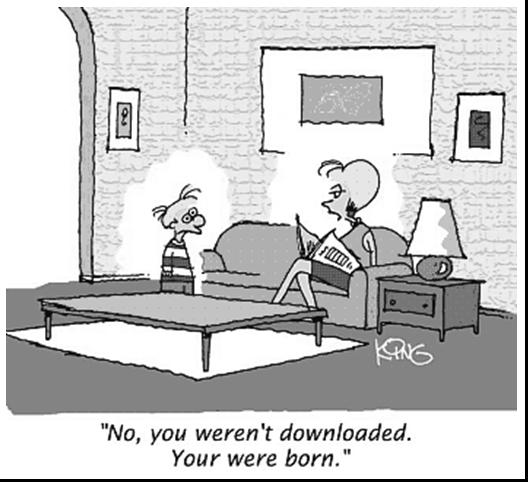
\includegraphics[width=.5\textwidth]{fig1.jpg}
\caption{A typical figure}
\label{fig:exampleFig1}
\end{figure}

\begin{figure}[ht]
\centering
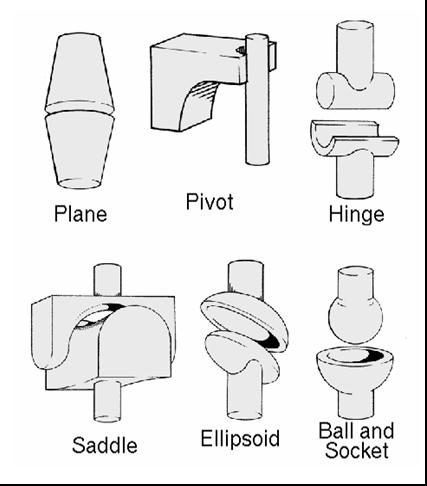
\includegraphics[width=.3\textwidth]{fig2.jpg}
\caption{This figure is an example of a figure caption taking more than one
  line and justified considering margins mentioned in Section~\ref{sec:figs}.}
\label{fig:exampleFig2}
\end{figure}

In tables, try to avoid the use of colored or shaded backgrounds, and avoid
thick, doubled, or unnecessary framing lines. When reporting empirical data,
do not use more decimal digits than warranted by their precision and
reproducibility. Table caption must be placed before the table (see Table 1)
and the font used must also be Helvetica, 10 point, boldface, with 6 points of
space before and after each caption.

\begin{table}[ht]
\centering
\caption{Variables to be considered on the evaluation of interaction
  techniques}
\label{tab:exTable1}
\smallskip
\begin{tabular}{|l|c|c|}
\hline
& Value 1 & Value 2\\[0.5ex]
\hline
&&\\[-2ex]
Case 1 & 1.0 $\pm$ 0.1 & 1.75$\times$10$^{-5}$ $\pm$ 5$\times$10$^{-7}$\\[0.5ex]
\hline
&&\\[-2ex]
Case 2 & 0.003(1) & 100.0\\[0.5ex]
\hline
\end{tabular}
\end{table}

\section{Images}

All images and illustrations should be in black-and-white, or gray tones,
excepting for the papers that will be electronically available (on CD-ROMs,
internet, etc.). The image resolution on paper should be about 600 dpi for
black-and-white images, and 150-300 dpi for grayscale images.  Do not include
images with excessive resolution, as they may take hours to print, without any
visible difference in the result. 

\section{References}

Bibliographic references must be unambiguous and uniform.  We recommend giving
the author names references in brackets, e.g. \cite{knuth:84},
\cite{boulic:91}, and \cite{smith:99}.

The references must be listed using 12 point font size, with 6 points of space
before each reference. The first line of each reference should not be
indented, while the subsequent should be indented by 0.5 cm.

\bibliographystyle{sbc}
\bibliography{sbc-template}

\end{document}
